% common part for every lection

\documentclass{beamer}

\usetheme{Warsaw}
\usefonttheme[onlylarge]{structurebold}
\setbeamerfont*{frametitle}{size=\normalsize,series=\bfseries}
\setbeamertemplate{navigation symbols}{}

\usepackage{pdfpages}
\usepackage{soul}
\usepackage{ucs}

% encoding settings
\usepackage[T2A]{fontenc}
\usepackage{xltxtra}
\usepackage{hyperref}
\usepackage{polyglossia}
\usepackage{xecyr}

\setdefaultlanguage{russian}

% fonts settings
\usepackage{fontspec}
\setmainfont[Ligatures=TeX]{CMU Serif}                 % Computer Modern Unicode font
\setsansfont[Ligatures=TeX]{CMU Sans Serif}
\setmonofont{CMU Typewriter Text}

\usepackage{listings}
\lstset{frame=single,breaklines=true,language=sh}

% for strike-out text
\usepackage[normalem]{ulem}

% tabulation aka \tbs
\newcommand{\tbs}{\tt\char`\\}

% \regex for regular expressions
\newcommand{\regex}[1]{ %
\expandafter{$\ulcorner{\color{blue}\texttt{#1}}\lrcorner$} %
}

% \qatrainingtitle
\newcommand{\qatrainingtitle}[2] {%
\title[SaM Solutions. Linux QA Training] %
{ %
  Часть #1.\\%
  #2 %
}

}

\newcommand{\firstframe}{ %
\begin{frame} %
  \titlepage %
\end{frame} %
}

\author[Author, Vlad Shakhov]{Влад 'mend0za' Шахов\\Linux \& Embedded Team Leader}

\institute[SaM Solutions]
{
  Linux \& Embedded Department
}

\date[Dec 2012]

\subject{Linux QA training}

\pgfdeclareimage[height=1.5cm]{sam-solutions-logo}{clipart/sam-solutions-elinux}

\logo{\pgfuseimage{sam-solutions-logo}}

\graphicspath{{./clipart/}}




\title[SaM Solutions. Linux QA Training]
{
  Часть 3.\\
  Файловая система, введение
}

\begin{document}

\firstframe

\section{Общие сведения}
\begin{frame}{Определения}
  \begin{itemize}
    \item В UNIX (и Linux) файлы организованы в виде \emph{единой древовидной структуры} (дерева), называемой \alert{файловой системой}.
    \item \alert{Каждый файл имеет имя}, определяющее его расположение в дереве FS.
    \item Корнем дерева является \alert{корневой каталог} (root directory), имеющий имя \alert{"/"}.
  \end{itemize} \pause

  \begin{itemize}
    \item \alert{полный путь} начинается с \alert{/}(корневого каталога), каталоги разделяются также \alert{/}. \newline
      Пример: /home/user/.ssh/authorized\_key
    \item \alert{относительный путь} - от текущего каталога \newline
      Примеры: ../user10/.bashrc; ./script; ls script
  \end{itemize}

\end{frame}

\subsection{Навигация по FS}
\begin{frame}{Навигация в командной строке (shell)}
  Для каждой запущенной программы (в том числе и shell) в системе определен \alert{текущий каталог}. 
  \begin{itemize} 
    \item \alert{pwd}\footnote{см также переменные окружения \alert{PWD} и \alert{OLDPWD}} - получить текущий каталог
    \item \alert{cd [папка]}\footnote{\alert{cd} без параметров - возврат в домашний каталог} - сменить каталог
    \item \alert{cd -}\footnote{Используется значение переменной \alert{OLDPWD}} - вернуться в предыдущий каталог
    \item \alert{ls [папка]}\footnote{\alert{ls} без параметров - просмотр текущего каталога} - просмотр списка файлов
    \item \alert{ls -l [папка]} - длинный листинг (c подробностями)
  \end{itemize}
\end{frame}

\subsection{Примеры деревьев Unix FS}

\begin{frame}{Дерево файловой системы - простое}
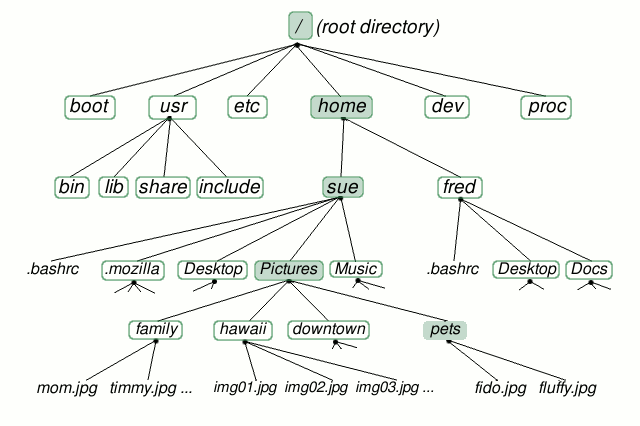
\includegraphics[height=8cm]{filesystem} 
\end{frame}

\begin{frame}{Дерево файловой системы - среднее}
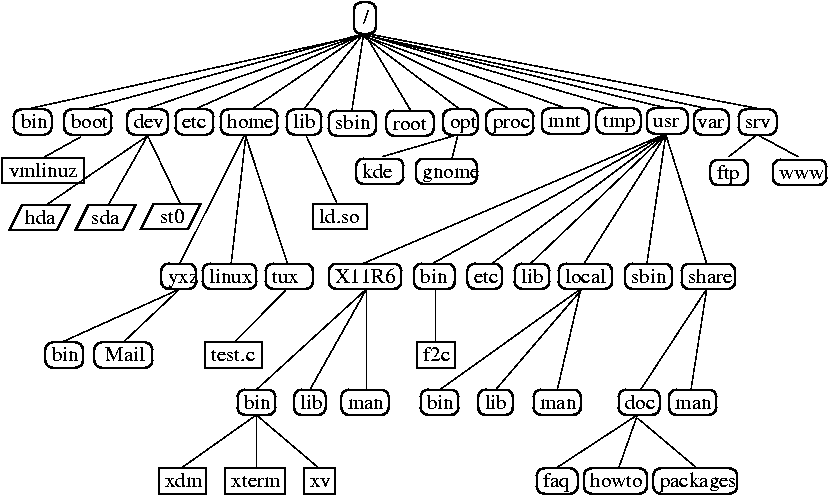
\includegraphics[height=7cm]{filesystem2} 
\end{frame}

\begin{frame}{Дерево файловой системы - сложное}
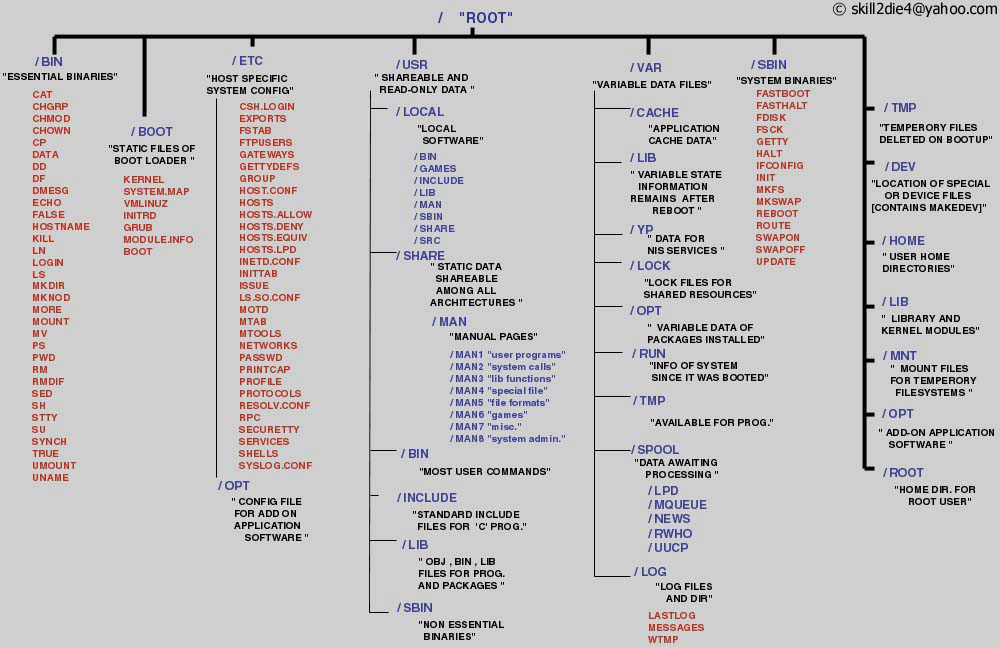
\includegraphics[height=7cm]{filesystem3} 
\end{frame}

\subsection{VFS}

\begin{frame}{Детали реализации}
  \begin{itemize}
    \item \alert{VFS - virtual file system} - файлы и каталоги отображаются в единое дерево, независимо от их физического расположения.
  \end{itemize}
  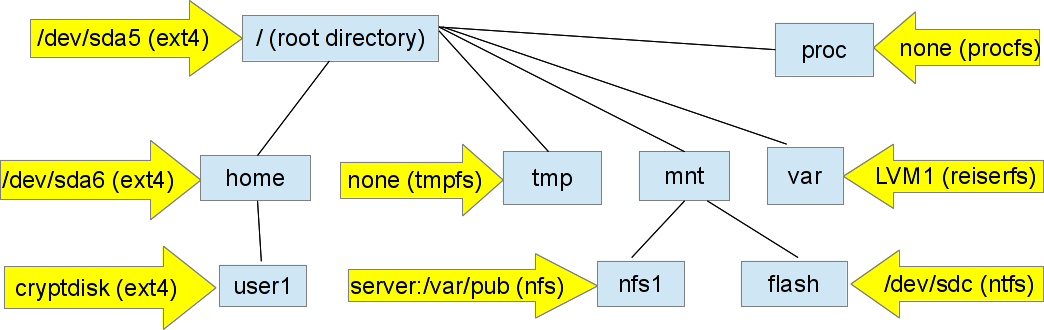
\includegraphics[height=3.5cm]{vfs-and-devices}
\end{frame}

\begin{frame}{Монтирование}
  \begin{itemize}
    \item \alert{Монтирование} - процесс отображения содержимого устройства в указанную папку файловой системы.
    \item Команды:
      \begin{itemize}
	\item монтировать - ( \alert{mount} ) 
	\item размонтировать ( \alert{umount} )
      \end{itemize}
    \item \alert{mount} без параметров - вывести список уже подключенных файловых систем
  \end{itemize}
  
\end{frame}

\section{Типы файлов}

\begin{frame}{Типы файлов в Unix}
  Для пользователя:
  \begin{itemize}
    \item \alert{Обычные файлы (regular file)}: .bashrc, /bin/bash
    \item \alert{Каталоги (directory)}: /home/user1, /usr, /, /usr/local  \pause
    \item \alert{Символические ссылки (symbolic links)}: /bin/sh, /dev/stdout
  \end{itemize} \pause
  Для администратора:
  \begin{itemize}
    \item \alert{Файлы устройств (device special file)}: 
      \begin{itemize}
	\item \alert{блочные}: /dev/sda5, /dev/loop0, /dev/sr0
	\item \alert{символьные}: /dev/null, /dev/mem, /dev/tty
      \end{itemize}
  \end{itemize} \pause 
  Для программиста:
  \begin{itemize}
    \item \alert{FIFO (named pipe)}: /dev/xconsole
    \item \alert{Socket}: /dev/log
  \end{itemize}

\end{frame}


\begin{frame}{Практика: определение типа файла}

  \begin{itemize}
    \item Используем \alert{ls -l}
      \lstinputlisting{samples/ls-l}
      Первая колонка, первый символ \pause

    \item Определение типа файла: \alert{file}
      \lstinputlisting{samples/file-usage}
  \end{itemize} 
\end{frame}

\subsection{Работа с обычными файлами}


\begin{frame}{Просмотр обычных файлов}
  %\frametitle{Просмотр обычных файлов}
  \begin{itemize}
    \item Просмотр текста:
      \begin{itemize} 
	\item \alert{cat} - вывести на stdout\footnote{Для двоичных файлов: чревато порчей настроек терминала} \pause
	\item \alert{more} - вывести, разбив на страницы
	\item \alert{less}\footnote{может отсутствововать в стандартной поставке} - \alert{more} на стероидах, с прокруткой, поиском 
      \end{itemize} \pause
    \item Просмотр двоичных данных:
      \begin{itemize} 
	\item \alert{od} - дамп файла в не-текстовых форматах
\lstinputlisting[frame=single,basicstyle=\tiny]{samples/od}
        \item \alert{strings} - извлечь текстовые строки из двоичных файлов
      \end{itemize}
  \end{itemize}

\end{frame}


\begin{frame}[fragile]{Создание (текстовых) файлов}
  \pause
  \begin{enumerate}
    \item Любимым редактором: \alert{vi/vim}, \alert{nano}, \alert{mcedit} \pause
    \item \alert{echo}
\begin{lstlisting}
echo какой-то текст >file
\end{lstlisting}\pause
    \item \alert{cat} с перенаправлением\footnote{До ``конца ввода'', т.е. нажатия Ctrl+D}
\lstinputlisting[basicstyle=\small]{samples/cat-input-file} \pause
    \item \alert{touch} - создать пустой файл
\begin{lstlisting}
~$ touch file4
~$
\end{lstlisting}
  \end{enumerate}
\end{frame}

\subsection{Операции над каталогами}

\begin{frame}[fragile]{Операции над каталогами (и файлами)}
  \begin{itemize}
    \item \alert{mkdir} - создать каталог
\begin{lstlisting}
~$ mkdir dir1 /tmp/somedir
~$ mkdir -p dir/and/existant/parts/in/path
\end{lstlisting} \pause
    \item \alert{rmdir} - удалить (пустой) каталог
\begin{lstlisting}
~$ rmdir dir1 /tmp/somedir
~$ rmdir -p deep/empty/dir/structure/
\end{lstlisting} \pause
    \item \alert{cp} - копирование файлов\footnotemark[8]
    \item \alert{mv} - перемещение и переименование файлов
    \item \alert{rm} - удаление файлов\footnotemark[17] 
\begin{lstlisting}
~$ rm -rf dir1 /tmp/somedir
~$ rm f*
\end{lstlisting} \pause
  \end{itemize}
\footnotetext[8]{с ключом \alert{-r}) и каталогов}
\end{frame}

% TODO - слайд про hardlinks и symlinks

\end{document}
